\documentclass[11pt]{article}

% NeurIPS 2024 style
\usepackage[preprint]{neurips_2024}

% Packages
\usepackage[utf8]{inputenc}
\usepackage{amsmath,amssymb,amsfonts}
\usepackage{graphicx}
\usepackage{booktabs}
\usepackage{array}
\usepackage{hyperref}
\usepackage{xcolor}

\hypersetup{
  colorlinks=true,
  linkcolor=black,
  citecolor=black,
  urlcolor=black
}

% Spacing overrides
\emergencystretch=2em
\setlength{\parskip}{3pt plus 1pt minus 1pt}
\setlength{\floatsep}{8pt plus 2pt minus 2pt}
\setlength{\textfloatsep}{10pt plus 3pt minus 3pt}
\setlength{\intextsep}{8pt plus 2pt minus 2pt}
\setlength{\abovecaptionskip}{4pt}
\setlength{\belowcaptionskip}{2pt}
% Section heading spacing (no titlesec needed)
\makeatletter
\renewcommand\section{\@startsection{section}{1}{\z@}%
  {-18pt \@plus -4pt \@minus -2pt}%
  {6pt \@plus 2pt}%
  {\normalfont\large\bfseries}}
\renewcommand\subsection{\@startsection{subsection}{2}{\z@}%
  {-12pt \@plus -2pt \@minus -2pt}%
  {4pt \@plus 1pt}%
  {\normalfont\normalsize\bfseries}}
\renewcommand\subsubsection{\@startsection{subsubsection}{3}{\z@}%
  {-6pt \@plus -1pt \@minus -1pt}%
  {2pt}%
  {\normalfont\normalsize\itshape}}
\makeatother

% Custom commands
\newcommand{\sgmvpi}{$(S, G, E, V, M, \pi)$}
\newcommand{\framework}{\textsc{SciAgent}}

% Title
\title{\textbf{Formalizing AI Scientist Systems:\\
A Unified Framework for Automated Scientific Discovery}}

\author{
  Jaesol Shin\\
  \small{WeDataLab}\\
  \texttt{ysys143@wedatalab.com}
}

\date{May 2026}

\begin{document}

\maketitle

\begin{abstract}
The emergence of end-to-end systems capable of automating hypothesis generation, experiment execution, and knowledge synthesis represents a significant change in how science is conducted. Despite rapid empirical progress, \emph{AI Scientist} systems lack a unifying formal framework, which makes principled comparison across architectures and scientific domains difficult. We propose \framework{}, a six-component framework \sgmvpi{} comprising the \textbf{S}earch space, hypothesis \textbf{G}enerator, \textbf{E}xperiment executor, \textbf{V}alidator, \textbf{M}emory, and search \textbf{P}olicy ($\pi$), grounded in the theory of Partially Observable Markov Decision Processes (POMDPs) and Bayesian Experimental Design (BED). We apply this framework to analyze core AI Scientist systems and their instantiations across seven scientific domains (mathematics, physics, chemistry, materials science, biology, social science, and computer science), and separately examine a complementary artifact infrastructure proposal that addresses the output format and verification layer of such systems. Our analysis surfaces three persistent open problems: (1) the non-automatability of novelty evaluation, which remains dependent on human judgment despite multi-layer automated proxies; (2) the absence of BED-optimal search policies, despite the theoretical availability of tractable approximations; and (3) the underdevelopment of semantic memory $M_s$, whose absence prevents accumulated experimental experience from improving future search. We show that the completeness of the validator $V$ is the single most consequential design variable: it determines whether closed-loop autonomous operation is feasible in each domain, and current AI Scientist systems can be read as a progression toward more complete validators.
\end{abstract}

\section{Introduction}

The pursuit of automated scientific discovery---systems that independently generate hypotheses, design and execute experiments, and synthesize new knowledge---has accelerated with the maturation of large language models (LLMs). Early demonstrations such as Coscientist~\citep{boiko2023emergent} showed that LLM-based agents could autonomously plan and execute chemical syntheses. Subsequent systems including The AI Scientist~\citep{lu2024aiscientist} and Agent Laboratory~\citep{schmidgall2025agentlab} extended this vision to the full research cycle: from literature survey and hypothesis generation to code execution, manuscript writing, and automated peer review. Most recently, systems such as Aletheia~\citep{google2026aletheia} have begun to engage with research-level mathematical problems. In parallel, proposals such as Agent-Native Research Artifacts~\citep{liu2026lasthuman} address a complementary problem: what the \emph{output} of AI Scientist systems should look like, and how it can be independently verified.

Despite this empirical momentum, the field lacks a shared formal vocabulary. Each system introduces its own architecture with bespoke terminology, making systematic comparison difficult. Questions that bear directly on practical deployment---\textit{What determines whether a system can operate in a closed loop? Why does autonomous novelty evaluation fail consistently? What is the theoretical optimum for the search policy?}---remain unanswered in the literature.

We address these gaps by making three contributions:

\begin{enumerate}
  \item We propose \framework{}, a formal framework \sgmvpi{} that decomposes any AI Scientist system into six components and connects it to the theoretical literature on POMDPs and Bayesian Experimental Design (Section~\ref{sec:framework}).
  \item We apply \framework{} to analyze four core AI Scientist systems (Section~\ref{sec:core}), a complementary artifact infrastructure proposal (Section~\ref{sec:ara}), and domain-specific instantiations across six scientific fields (Section~\ref{sec:domains}).
  \item We identify three open problems that constrain progress across all current systems (Section~\ref{sec:openproblems}).
\end{enumerate}

\noindent\textbf{Scope.} This survey covers systems whose primary goal is automated scientific \emph{discovery}---generating new knowledge through hypothesis-experiment-validation cycles. We explicitly exclude systems that apply AI as a specialized tool within a human-conducted research pipeline (e.g., AlphaFold~\citep{jumper2021alphafold} for structure prediction), as these lack the hypothesis-generation and iterative search components central to our framework.

\section{Background}
\label{sec:background}

\subsection{POMDP Formulation of Scientific Discovery}

Following the POMDP formulation~\citep{kaelbling1998pomdp}, we model AI Scientist systems as \emph{partially observable Markov decision processes}. The true state $s \in \mathcal{S}$ corresponds to the unknown structure of nature (e.g., the correct physical law, the optimal molecular configuration). Because $s$ is never directly accessible, the system maintains a belief state $b(s)$ updated by observations $o \in \Omega$ obtained through experiments.
\par

Formally, an AI Scientist POMDP is the tuple $(\mathcal{S}, \mathcal{A}, T, R, \Omega, \mathcal{O}, \gamma)$, where $\mathcal{A}$ is the action space (hypothesis generation, experiment execution), $T: \mathcal{S} \times \mathcal{A} \rightarrow \Delta(\mathcal{S})$ is the transition function, $R: \mathcal{S} \times \mathcal{A} \rightarrow \mathbb{R}$ is the reward (scientific value of discovery), and $\mathcal{O}: \mathcal{S} \times \mathcal{A} \rightarrow \Delta(\Omega)$ is the noisy observation process.

This formulation departs from standard POMDPs in three ways specific to scientific discovery: (1) the reward function $R$ is not pre-specified, as scientific significance cannot be defined a priori; (2) the state space $\mathcal{S}$ is unbounded and open-ended; and (3) the transition function $T$ is non-stationary, since accumulated knowledge changes the frontier of valuable exploration.

\subsection{Bayesian Experimental Design}

Bayesian Experimental Design (BED)~\citep{chaloner1995bayesian,rainforth2024modern} provides a principled basis for the search policy $\pi$. The optimal policy selects the experiment $d^*$ that maximizes the Expected Information Gain (EIG):

\begin{equation}
  d^* = \arg\max_{d \in \mathcal{D}}\; \mathrm{EIG}(d) = \arg\max_{d}\; \mathbb{E}\left[H(\theta) - H(\theta \mid y, d)\right]
  \label{eq:eid}
\end{equation}

where $H(\theta)$ is the prior entropy over parameters $\theta$ and $H(\theta \mid y, d)$ is the expected posterior entropy after observing outcome $y$ under experiment $d$. The two frameworks are complementary rather than competing: POMDP provides the structural formulation of the decision problem, while BED provides the normative criterion for the policy $\pi$.

Recent work has shown that EIG can be approximated via variational methods~\citep{foster2019variational}, amortized neural policies~\citep{foster2021dad}, and reinforcement learning~\citep{blau2022rl}. Despite their theoretical availability, no current AI Scientist system explicitly implements EIG-optimal policies---a gap we identify as a central open problem.

\section{Related Work}
\label{sec:related}

\textbf{AI Scientist surveys and system papers.} The literature on AI Scientist systems has grown rapidly but lacks shared vocabulary. \citet{lu2024aiscientist} propose the first closed-loop end-to-end system and provide qualitative characterization of their own components, but do not offer a formal framework for cross-system comparison. \citet{schmidgall2025agentlab} focus on co-pilot design and evaluate cost reduction against human baselines. \citet{boiko2023emergent} demonstrate tool-augmented autonomous synthesis but do not model the discovery loop. \citet{si2024novelideas} conduct a large-scale human study on LLM idea generation quality, establishing baselines for novelty evaluation; \citet{baek2024researchagent} propose iterative literature-conditioned ideation. Neither provides a framework that unifies search, execution, validation, and memory. The closest precursor to our framework is the qualitative discussion in \citet{lu2026aiscientist}, which introduces the concept of open-ended archives and replication nodes but does not formalize these as components of a general system.

\textbf{Theoretical foundations: POMDP and BED.} The POMDP formulation of decision-making under partial observability is classical~\citep{kaelbling1998pomdp}. Bayesian Experimental Design formalizes the optimal experiment selection criterion~\citep{chaloner1995bayesian}; recent work provides tractable approximations via variational inference~\citep{foster2019variational}, amortized neural policies~\citep{foster2021dad}, and reinforcement learning~\citep{blau2022rl}. We connect these two bodies of work: POMDP provides the structural formulation while BED provides the normative policy criterion. To our knowledge, no prior work explicitly applies BED as a design target for AI Scientist search policies.

\textbf{Domain-specific AI science systems.} Substantial prior work applies AI to scientific problems without proposing general frameworks: FunSearch~\citep{romera2023funsearch} and DeepSeek-Prover~\citep{xin2024deepseek} in mathematics; AI Feynman~\citep{udrescu2020afeynman} in physics; ChemCrow~\citep{bran2023chemcrow} and ChemReasoner~\citep{sprueill2024chemreasoner} in chemistry; BioPlanner~\citep{odonoghue2023bioplanner} in biology; AutoML-Zero~\citep{real2020automlzero} in computer science. We treat these as \framework{} component instantiations, enabling principled cross-domain comparison.

\textbf{Formal models of science.} \citet{taniguchi2024cpc} propose Collective Predictive Coding as a Model of Science (CPC-MS), recasting scientific activity as decentralized Bayesian inference across a community of agents with diverse priors. Their framework maps directly onto \framework{} components: hypothesis generation as internal-representation inference $q(z^k \mid w, o^k)$, experimentation as action-conditioned observation $p(o \mid z, a)$, peer review as collective consensus $q(w \mid \{z^k\})$, and search policy as expected free energy minimization. The key distinction is scope: CPC-MS is a \emph{collective} and \emph{social} model, while \framework{} is a \emph{single-system} and \emph{modular} decomposition. Notably, CPC-MS explicitly analyzes Lu et al.'s AI Scientist and argues that it automates only a single researcher's loop while leaving the collaborative peer-review and consensus layer unaddressed---motivating the collective extension we discuss in Section~\ref{sec:discussion}.

\textbf{Research artifact infrastructure.} \citet{liu2026lasthuman} propose Agent-Native Research Artifacts (ARA) as a structured output format and verification protocol for AI-produced research. We position this contribution separately from end-to-end AI Scientist systems, as it addresses the artifact layer rather than the discovery loop, and discuss its implications for the $V$ and $M_s$ components of \framework{} in Sections~\ref{sec:ara} and~\ref{sec:openproblems}.

\section{The \framework{} Framework}
\label{sec:framework}

We define an AI Scientist system as a tuple \sgmvpi{} with the following components:

\begin{equation}
  \text{\framework{}} = (S,\; G,\; E,\; V,\; M,\; \pi)
\end{equation}

\begin{description}
  \item[$S$: Search Space] The set of candidate hypotheses, programs, molecules, experimental conditions, or other objects subject to exploration. $S$ may be static or dynamically expanding (open-ended).

  \item[$G: M \times S \rightarrow h$: Hypothesis Generator] A function that proposes new candidate $h \in S$ conditioned on accumulated memory $M$ and the current state of the search space. $G$ may involve LLM generation, evolutionary mutation, or symbolic search.

  \item[$E: h \times P \rightarrow o$: Experiment Executor] A function that executes hypothesis $h$ under protocol $P$ to produce observation $o$. The fidelity of $E$ ranges from fast computational simulation (low cost, potential surrogate error) to physical wet-lab execution (high cost, ground truth).

  \item[$V: o \rightarrow r$: Validator] A function that assigns a reward signal $r$ to observation $o$. We distinguish four layers of $V$:
    \begin{align*}
      V_\text{syntax}   &: o \rightarrow \{\text{pass}, \text{fail}\} & \text{(deterministic, fast)}\\
      V_\text{semantic} &: o \rightarrow r \in [0,1]                  & \text{(LLM-based, stochastic)}\\
      V_\text{empirical}&: o \rightarrow r                            & \text{(reproduction-based)}\\
      V_\text{human}    &: o \rightarrow \{\text{novel}, \text{significant}\} & \text{(non-automatizable)}
    \end{align*}

  \item[$M$: Memory] Structured as $(M_e, M_s, M_p)$. $M_e$ (episodic) stores individual records $(h_i, o_i, r_i)$; $M_s$ (semantic) stores distilled knowledge patterns; $M_p$ (procedural) stores learned protocols. The structure of $M$ directly determines the quality of $G$ and $\pi$.

  \item[$\pi: b(S) \times M \rightarrow h$: Search Policy] The decision rule for selecting the next hypothesis. The belief state $b(S)$ is updated after each experiment. In the BED interpretation, $\pi^* = \arg\max_d \mathrm{EIG}(d)$ (Equation~\ref{eq:eid}). In practice, current systems use policies ranging from reactive (ReAct) to greedy to tree search.
\end{description}

\noindent The operational loop is:
\begin{align}
  \pi(b, M) &\;\rightarrow\; G(M_s, S) \;\rightarrow\; E(h, P) \;\rightarrow\; V(o) \nonumber\\
            &\;\rightarrow\; M \mathrel{+}= (h, o, r) \;\rightarrow\; b(S) \text{ update} \;\rightarrow\; \text{repeat}
\end{align}

We further introduce $H \in [0,1]$ as an auxiliary parameter denoting the degree of human intervention: $H=0$ for fully autonomous systems and $H=1$ for systems in which humans assume the role of $G$ or $\pi$.

\section{Analysis of Core AI Scientist Systems}
\label{sec:core}

We apply \framework{} to four core systems that propose or implement end-to-end automated research pipelines (Sections~\ref{sec:coscientist}--\ref{sec:agentlab}), followed by one artifact infrastructure proposal that addresses the output format and verification layer of such systems (Section~\ref{sec:ara}). For each end-to-end system, we characterize the six components and assess three quality dimensions: (A) novelty claim mechanism, (B) closed-loop completeness, and (C) scientific quality assurance.

\subsection{Coscientist}
\label{sec:coscientist}

\citet{boiko2023emergent} demonstrate that GPT-4 can autonomously plan and physically execute chemical syntheses via a tool-augmented ReAct loop.

\begin{table}[h]
\centering
\small
\begin{tabular}{@{}lp{9cm}@{}}
\toprule
Component & Instantiation \\
\midrule
$S$ & Known chemical reaction space (reproduction, not discovery) \\
$G$ & Human-provided task $\rightarrow$ GPT-4 Planner steps; no autonomous ideation \\
$E$ & Tool calls (web, docs, code) + RoboRXN physical synthesis; analytical characterization delegated to human \\
$V$ & $V_\text{human}$ only: author inspection + single GC-MS measurement \\
$M$ & Session conversation history; no cross-session persistence \\
$\pi$ & Greedy ReAct: next tool action conditioned on current context; no branching \\
\bottomrule
\end{tabular}
\caption{Coscientist \sgmvpi{} mapping.}
\end{table}

\noindent\textbf{(A) Novelty.} No novelty measurement mechanism exists; all synthesis targets are known compounds. The system's novelty claim concerns architectural capability, not scientific discovery.

\noindent\textbf{(B) Loop.} The loop does not close: there is no hypothesis $\rightarrow$ experiment $\rightarrow$ new hypothesis cycle. Physical execution succeeds, but measurement results are not fed back to the agent.

\noindent\textbf{(C) Quality.} Single GC-MS measurement with no replication, no statistical testing, and no public data release (withheld for safety reasons). The authors note that multi-run variance analysis is future work.

\subsection{The AI Scientist (Sakana AI)}
\label{sec:aisci-sakana}

\citet{lu2024aiscientist} propose the first system to close the full research loop: ideation, experimentation, manuscript writing, and automated peer review.

\begin{table}[h]
\centering
\small
\begin{tabular}{@{}lp{9cm}@{}}
\toprule
Component & Instantiation \\
\midrule
$S$ & ML research idea space, implicitly bounded by seed code templates \\
$G$ & LLM ideation conditioned on archive $M_e$; Semantic Scholar API (10 rounds) similarity filter \\
$E$ & Aider code agent $\rightarrow$ Python execution; max 4 retries, 7200s timeout \\
$V$ & $V_\text{semantic}$: GPT-4o reviewer (NeurIPS guidelines, 5-ensemble); BalAcc 0.65 vs.\ human 0.66 \\
$M$ & $M_e$: idea archive with title, scores, results; no $M_s$ or $M_p$ \\
$\pi$ & Greedy: generate hypothesis dissimilar to archive; no long-horizon planning \\
\bottomrule
\end{tabular}
\caption{The AI Scientist (Sakana 2024) \sgmvpi{} mapping.}
\end{table}

\noindent\textbf{(A) Novelty.} LLM self-scores each idea on novelty (1--10 scale). The authors acknowledge systematic over-estimation bias and that ``judgments by LLMs can often have bias''~\citep{lu2024aiscientist}. Importantly, the authors state: \textit{``we do not recommend taking the scientific content of this version of The AI Scientist at face value.''}

\noindent\textbf{(B) Loop.} The first genuinely closed loop: review scores feed into the next ideation cycle via $M_e$. However, $\pi$ is greedy and does not improve with archive growth.

\noindent\textbf{(C) Quality.} Statistical rigor is weak: seeds and confidence intervals are not enforced. An early system version hallucinated ablation tables. Safety violations were observed, including a subprocess that indefinitely spawned Python processes and an agent that attempted to extend its own timeout.

\subsection{The AI Scientist (Nature 2026)}
\label{sec:aisci-nature}

\citet{lu2026aiscientist} extend the Sakana system with agentic tree search and an open-endedness archive, achieving the first AI-authored manuscript accepted at a peer-reviewed workshop (ICLR 2025 ICBINB, score 6.33).

\begin{table}[h]
\centering
\small
\begin{tabular}{@{}lp{9cm}@{}}
\toprule
Component & Instantiation \\
\midrule
$S$ & Open-endedness archive (dynamic $S$); idea novelty checked against Semantic Scholar (20 rounds) \\
$G$ & LLM conditioned on $S_\text{archive}$ and $M_e$; Semantic Scholar similarity filter \\
$E$ & 4-phase agentic tree search; VLM critique on figures; Aider with 4 retries \\
$V$ & $V_\text{empirical}$: replication nodes (mean $\pm$ s.d.); $V_\text{semantic}$: automated reviewer (BalAcc 0.69); $V_\text{human}$: ICLR reviewers \\
$M$ & $M_e$: tree nodes; $M_s$: open-endedness archive; replication statistics \\
$\pi$ & Best-first tree search: GPT-4o scores nodes on metrics, training dynamics, and figure quality \\
\bottomrule
\end{tabular}
\caption{The AI Scientist (Nature 2026) \sgmvpi{} mapping.}
\end{table}

\noindent\textbf{(A) Novelty.} Three-layer validation: self-score, API filter, and actual peer review. Automated reviewer performance: balanced accuracy 0.69 (vs.\ human 0.66), F1 0.62 (vs.\ human 0.49), with no significant difference from human accuracy on both pre-cutoff ($p=0.319$) and post-cutoff ($p=0.921$) data. Limitations remain: hallucinated citations and the inherent risk that pretraining data contaminates novelty judgments.

\noindent\textbf{(B) Loop.} The most complete closed loop to date: tree search provides reward-guided $\pi$, VLM critique creates within-$E$ feedback, and replication nodes enforce statistical validation.

\noindent\textbf{(C) Quality.} Bootstrap CIs (5,000 replicates) and z-tests are reported. Hallucinated citations remain a documented failure mode; the workshop acceptance rate (70\%) differs from the main conference rate (32\%), limiting the significance of the peer review validation.

\subsection{Agent Laboratory}
\label{sec:agentlab}

\citet{schmidgall2025agentlab} adopt a co-pilot design in which human researchers provide the research direction, and LLM agents execute the research pipeline (literature review, experimentation, manuscript writing).

\begin{table}[h]
\centering
\small
\begin{tabular}{@{}lp{9cm}@{}}
\toprule
Component & Instantiation \\
\midrule
$S$ & Human-provided research direction (constrained $S$; no autonomous ideation) \\
$G$ & Human idea $\rightarrow$ PhD agent elaborates via literature review \\
$E$ & mle-solver: EDIT/REPLACE + LLM reward scoring + self-reflection + top-program pool \\
$V$ & $V_\text{semantic}$: NeurIPS LLM reviewer; systematic over-estimation (+2.3 points vs.\ human) \\
$M$ & Literature collection ($M_e$); no $M_s$ or $M_p$ \\
$\pi$ & Co-pilot: human; autonomous: fixed sequential; paper refinement $\rightarrow$ backward edge to prior phase \\
\bottomrule
\end{tabular}
\caption{Agent Laboratory \sgmvpi{} mapping.}
\end{table}

\noindent\textbf{(A) Novelty.} Novelty is handled by having the human provide the research direction. The system explicitly states: \textit{``the strongest research systems would combine human-guided ideation with LLM-based workflows''}~\citep{schmidgall2025agentlab}.

\noindent\textbf{(B) Loop.} The only backward edge is from paper refinement to prior phases. The mle-solver contains the most sophisticated within-$E$ micro-loop of any system analyzed. Termination is heuristic (max steps or timeout).

\noindent\textbf{(C) Quality.} The automated reviewer over-estimates quality by +2.3 points on average compared to human PhD students. A documented hallucination case: GPT-4o fabricated hyperparameter values (``learning rate 0.001, batch size 32 over 50 epochs'') that were never actually tested.

\subsection{Comparative Summary}
\label{sec:core-summary}

Table~\ref{tab:core-comparison} synthesizes the four end-to-end systems along the key dimensions identified by \framework{}.

\begin{table}[h]
\centering
\small
\setlength{\tabcolsep}{4pt}
\begin{tabular}{@{}lcccc@{}}
\toprule
& \textbf{Coscientist} & \textbf{AI Sci.\ (2024)} & \textbf{AI Sci.\ (2026)} & \textbf{AgentLab} \\
\midrule
Novelty measure   & None         & LLM self-score & 3-layer         & Human-delegated \\
Loop closed?      & No           & Yes (greedy)   & Yes (tree)      & Partial         \\
$\pi$ type        & ReAct        & Greedy         & Tree search     & Human/seq.      \\
$V$ completeness  & $V_h$ only   & $V_s$          & $V_e+V_s+V_h$  & $V_s$ (biased)  \\
$M$ structure     & Ephemeral    & $M_e$          & $M_e+M_s$       & $M_e$           \\
$H$ (human role)  & G            & Low            & Low             & G+$\pi$         \\
\bottomrule
\end{tabular}
\caption{Comparative \framework{} analysis of four core AI Scientist systems. $V_s$=semantic, $V_e$=empirical, $V_h$=human.}
\label{tab:core-comparison}
\end{table}

\subsection{Artifact Infrastructure: Agent-Native Research Artifacts}
\label{sec:ara}

The four systems above address the internal structure of the AI Scientist loop. \citet{liu2026lasthuman} address a complementary problem: what the \emph{output} of that loop should look like, and how it can be independently verified. They propose Agent-Native Research Artifacts (ARA), a structured protocol that replaces the narrative paper with a four-layer file-system ontology: \texttt{/logic} (claims with explicit falsification criteria, hypotheses, related-work dependency graph), \texttt{/src} (typed kernel modules or full repository), \texttt{/trace} (exploration graph with five typed node types: question, decision, experiment, dead\_end, pivot), and \texttt{/evidence} (raw machine-readable results, withheld from verification agents to enable blind reproduction).

The motivation is quantitative: \citet{liu2026lasthuman} report that only 45.4\% of papers provide sufficient information for reproduction, and that 90.2\% of the dollar cost of extending a paper is consumed by failed rediscovery of methods already known to the original authors. ARA addresses this by making the full research process---including dead ends and pivots---a first-class published artifact.

ARA makes two direct contributions to the components of \framework{}. First, it addresses $V$ via the ARA Seal: a three-level automated verification credential combining $V_\text{syntax}$ (schema conformance and cross-layer reference integrity, seconds), $V_\text{semantic}$ (Rigor Auditor with a six-dimensional rubric, catching 82.6\% of seeded validity mutations), and $V_\text{empirical}$ (sandboxed directional reproduction). $V_\text{human}$ is retained for significance, novelty, and taste as an explicit design principle: \textit{``judgments of significance, novelty, and taste are reserved for human reviewers''}~\citep{liu2026lasthuman}. Second, the \texttt{/trace} layer addresses $M_e$ and $M_s$: forensic bindings link each claim to the experiment that supports it and to raw evidence files, externalizing the semantic structure of accumulated knowledge.

A key empirical finding bears on $\pi$: preserved failure traces (dead\_ends, pivots) in the \texttt{/trace} layer accelerated downstream agent performance in extension tasks, but the same traces also constrained more capable agents by anchoring them to prior solution paths. Richer $M_e$ does not monotonically improve $\pi$.

The paper positions ARA as a substrate rather than a system: ``ARA closes this gap not by replacing these tools but by providing the missing structural layer''~\citep{liu2026lasthuman}. In \framework{} terms, ARA specifies a standard output format for $E$ and input format for $G$, with the goal that when AI Scientist systems produce and consume ARAs rather than narrative PDFs, accumulated knowledge compounds at the artifact level rather than the sentence level.

\section{Domain Analysis}
\label{sec:domains}

We examine how \framework{} components are instantiated across seven scientific domains, revealing that the completeness of $V$ is the primary determinant of closed-loop feasibility.

\subsection{Mathematics}

Mathematics uniquely enables $V_\text{formal}$---a perfect oracle implemented by formal proof assistants such as Lean 4. This has direct consequences for $\pi$: because the reward signal is binary and noise-free, reinforcement learning is applicable without reward hacking.

\textbf{FunSearch}~\citep{romera2023funsearch} instantiates $S$ as the space of Python functions (short programs implementing priority heuristics), $G$ as LLM mutation conditioned on the best-so-far population, $E$ as deterministic sandboxed execution, and $V_\text{empirical}$ as the numerical score from a user-provided evaluator. The loop is fully closed; novelty is established via quantitative SOTA improvement.

\textbf{DeepSeek-Prover-V1.5}~\citep{xin2024deepseek} uses $S$ = Lean 4 tactic scripts, $E$ = Lean proof kernel (decidable), $V_\text{formal}$ = type-check success (perfect oracle), and $\pi$ = RMaxTS (UCB + intrinsic exploration reward) combined with RLPAF (reinforcement learning from proof assistant feedback). The noise-free $V$ enables stable RL without reward hacking.

\textbf{Aletheia}~\citep{google2026aletheia} takes the opposite approach: $S$ is natural language proof space, $V$ is a fallible LLM Verifier subagent, and $V_\text{human}$ remains the ground truth. Of 700 Erd\H{o}s problems attempted, human auditors rated only 13 (1.9\%) as ``meaningfully correct.'' The system explicitly identifies ``subconscious plagiarism''---pretraining data contamination masking as discovery---as a serious validity threat.

The key observation is that $S$ choice bifurcates mathematical AI Scientist paradigms: program-space ($V_\text{empirical}$ sufficient, full autonomy possible) vs.\ natural-language-proof-space ($V_\text{human}$ required, partial autonomy only).

\subsection{Physics}

\textbf{AI Feynman}~\citep{udrescu2020afeynman} encodes domain knowledge in $\pi$ rather than $G$: the search policy applies physics-specific heuristics (dimensional analysis, symmetry detection, separability) to progressively reduce the effective size of $S$. $M_e$ is absent---each mystery starts fresh. The loop is partially closed: there is no cross-mystery knowledge accumulation.

\textbf{Discovering Symbolic Models}~\citep{cranmer2020symbolic} uses a two-stage pipeline: GNN training ($G$ via inductive bias over interacting particle systems) followed by symbolic regression ($E$ via Eureqa genetic algorithm). The loop is fully open; discovered formulas do not feed back into GNN training. $V_\text{human}$ plays a decisive role: ``this formula is new to cosmologists.''

\textbf{Domain observation.} Physics law discovery requires $V$ to evaluate both numerical accuracy and interpretability (symbolic form). This dual requirement is absent in algorithm discovery (accuracy only) and is more demanding than mathematical construction (SOTA score only).

\subsection{Chemistry}

\textbf{ChemCrow}~\citep{bran2023chemcrow} is architecturally similar to Coscientist: tool-augmented ReAct with 18 APIs. The physical loop is open at the analytical measurement boundary---the robotic synthesizer executes reactions, but NMR, MS, and UV-Vis characterization remain human-delegated. $V_\text{semantic}$ (EvaluatorGPT) is shown to be unreliable: it cannot distinguish between correct and clearly incorrect GPT-4 outputs.

\textbf{ChemReasoner}~\citep{sprueill2024chemreasoner} introduces the strongest $M$ and $\pi$ of any domain paper analyzed: a tree-structured $M_e$ storing all visited (question, answer, reward) nodes, and a beam search $\pi$ (beam width $M=6$) that selects top-scoring nodes for expansion at each depth. $E$ is computational only (GNN surrogate, GemNet-dT), with DFT validation reserved for post-hoc verification. The authors document divergence between GNN predictions and DFT ground truth, confirming that $V$ is a surrogate with systematic error.

\textbf{Domain observation.} The wet-lab loop in chemistry is structurally open at the measurement boundary. Physical execution is achievable (ChemCrow, Coscientist); automated analytical characterization is not. ChemReasoner is the only chemistry system with a BED-adjacent $\pi$ (beam search over reward-ranked nodes).

\subsection{Materials Science}

Materials discovery presents a distinct $V$ profile: formation energy per atom computed via Density Functional Theory (DFT) serves as a near-perfect empirical oracle---computationally expensive but noise-free and ground-truth aligned---while physical synthesis constitutes a costly, human-mediated second validation layer.

\textbf{GNoME}~\citep{merchant2023gnome} (Graph Networks for Materials Exploration, DeepMind) scales this structure to 380 million hypothetical inorganic crystal structures. $G$ is a pair of Graph Neural Networks (GNNs) trained to predict thermodynamic stability: one structural GNN operating on known crystal prototypes and one compositional GNN operating on element combinations. $E$ is high-throughput DFT. $\pi$ is entropy-weighted uncertainty sampling: candidates where the GNN is most uncertain are prioritized for DFT evaluation, approximating an active learning policy over $b(S)$. $M_s$ grows as the GNN retrains on accumulated DFT outcomes; GNoME is one of the few systems where $G(M_s, S)$ genuinely improves with accumulated experiments.

\begin{table}[h]
\centering
\small
\begin{tabular}{@{}lp{9cm}@{}}
\toprule
Component & Instantiation \\
\midrule
$S$ & 380M hypothetical inorganic crystal structures \\
$G$ & Dual GNN (structural + compositional) predicts stability; retrained on DFT outcomes \\
$E$ & High-throughput DFT (computational); synthesis at collaborating labs (physical) \\
$V$ & $V_\text{empirical}$: formation energy / above-hull threshold (DFT); $V_\text{human}$: synthesis confirmation \\
$M$ & $M_e$: 460K prior DFT results; $M_s$: GNN weights updated each iteration \\
$\pi$ & Uncertainty sampling: prioritize high-entropy predictions for DFT \\
\bottomrule
\end{tabular}
\caption{GNoME \sgmvpi{} mapping.}
\end{table}

\noindent Key results: 2.2 million stable structures identified (83\% novel, precision 0.87), of which 736 were experimentally synthesized in collaboration with a robotic lab. The computational loop is closed; the synthesis loop remains open, with weeks-to-months latency for physical validation.

\textbf{Domain observation.} Materials science is the domain where $\pi$ most closely approximates BED theory. GNoME's uncertainty-sampling policy is structurally equivalent to information-gain maximization over a probabilistic stability model, closer to EIG-optimal than any system in other domains. The primary bottleneck is the DFT wall-time (hours per candidate), which limits the loop frequency but does not prevent closure.

\subsection{Biology}

\textbf{BioPlanner}~\citep{odonoghue2023bioplanner} contributes a pseudofunction abstraction that enables automatic evaluation of protocol-generation quality (function accuracy, argument precision, sequence order). The system's primary contribution is $V$ operationalization rather than $G$-$E$-$V$ loop closure. Wet-lab validation succeeds (E.\ coli culture executed without modification), but results are not fed back to the generator.

\textbf{AlphaFold 2}~\citep{jumper2021alphafold} is explicitly excluded from the \framework{} mapping: it is a discriminative predictor, not a hypothesis-experiment loop. $\pi$ is absent (recycling is a fixed 3-iteration refinement); $G$ performs no hypothesis generation; experimental feedback does not occur during inference. AlphaFold 2 represents a target capability that motivates AI Scientist development in biology rather than an instance of the pattern.

\subsection{Social Science}

Social science is unique in that LLMs substitute for $E$ (human subjects experiments). This creates a structural validity threat: when $G$ and $E$ share the same underlying model, the experiment executor may confirm the hypothesis generator's implicit biases.

\textbf{Automated Social Science}~\citep{manning2024automated} demonstrates that LLM-simulated experiments yield results directionally consistent with economic theory. However, LLMs systematically over-estimate effect magnitudes by 13.2$\times$ when queried directly, while simulation-based estimates are closer to theory. The system's $\pi$ is a full-factorial design over exogenous SCM variables; cross-scenario transition is not automated ($H$ intervenes at this boundary).

\textbf{Generative Agents}~\citep{park2023generative} provides E-infrastructure (memory stream + reflection + planning architecture) that subsequent systems use. It is not itself an AI Scientist system---the loop produces socially plausible behavior, not scientific discovery.

\textbf{Turing Experiments}~\citep{aher2023turing} serves as a meta-paper, measuring whether LLMs constitute valid $E$ for social science. Key finding: \emph{hyper-accuracy distortion}---stronger LLMs produce answers too accurate to simulate human population distributions. This identifies a fundamental constraint on $E$ fidelity in social science AI Scientist systems.

\subsection{Computer Science}

\textbf{AutoML-Zero}~\citep{real2020automlzero} evolves complete ML algorithms from primitive mathematical operations using a regularized evolutionary algorithm. $S$ = operation sequences (three components: Setup, Predict, Learn), $V_\text{empirical}$ = validation accuracy on proxy tasks, $\pi$ = tournament selection with aging regularization. The loop is fully closed and runs for millions of generations.

\textbf{Algorithm Discovery with LLMs}~\citep{sartori2024algodiscovery} uses LLMs as semantic mutation operators: instead of syntactic bit-flipping, the LLM understands the current program's logic and proposes meaningful variations. This reduces search space by orders of magnitude relative to blind evolutionary search.

\textbf{AutoKernel}~\citep{jaber2026autokernel} targets GPU kernel optimization, making $S$ the space of CUDA/Triton implementations and $V_\text{empirical}$ the measured runtime speedup on hardware. An LLM agent reads a structured optimization playbook ($M_p$), proposes code edits to the current kernel, and executes a five-stage correctness gate before benchmarking. $\pi$ is a keep/revert policy: edits that pass correctness checks and achieve $>$1.01$\times$ speedup are committed; others are rolled back via \texttt{git reset}. The loop runs unattended overnight (300--400 iterations per 10-hour run), achieving 2--5$\times$ kernel speedups at a $\sim$20\% per-iteration success rate.

AutoKernel represents the clearest example of $M_p$ (procedural memory) as a primary system component: the optimization playbook encodes expert heuristics---roofline model constraints, memory coalescing patterns, tiling strategies---in a structured format that guides $G$ without LLM hallucination of inapplicable strategies.

\subsection{Cross-Domain Summary}

Table~\ref{tab:domain-comparison} summarizes the \framework{} analysis across domains. The key finding is that $V$ completeness determines $\pi$ capability and closed-loop feasibility.

\begin{table}[h]
\centering
\small
\setlength{\tabcolsep}{4pt}
\begin{tabular}{@{}lccccp{2.6cm}@{}}
\toprule
Domain & $V$ type & $V$ reliability & Loop & $\pi$ & Primary bottleneck \\
\midrule
Math (formal) & $V_\text{formal}$ & Perfect oracle & Fully closed & RL/MCTS  & Pretraining contamination \\
Math (NL) & $V_\text{sem}+V_h$ & Imperfect & Partial & Seq.\ refine & Hallucination; plagiarism \\
Physics & $V_\text{emp}+V_h$ & Medium & None/partial & Deterministic & No cross-problem $M$ \\
Chemistry & $V_\text{emp}$ (surr.) & Medium & Comp.\ only & Beam & Wet-lab loop open \\
Materials & $V_\text{emp}$ (DFT) & High & Comp.\ closed & Uncert.\ samp. & DFT wall-time; synth.\ lag \\
Biology & $V_\text{emp}+V_h$ & Low--med & Partial & None & $V$ metrics insufficient \\
Social Sci. & Stat.\ test & Low--med & Partial & Factorial & Circular validity \\
CS / Algo. & $V_\text{emp}$ & High & Fully closed & Evol./LLM & Interpretability absent \\
\bottomrule
\end{tabular}
\caption{Cross-domain \framework{} analysis across seven domains. $V$ reliability refers to agreement with ground truth.}
\label{tab:domain-comparison}
\end{table}

% ---------------------------------------------------------------------------
\section{Illustrative Simulation: Validator Coverage and False Novelty}
\label{sec:simulation}
% ---------------------------------------------------------------------------

To make the consequences of $V$ incompleteness concrete, we construct a minimal agent-based simulation in which the degree of $V$ completeness is the only variable altered across conditions. We model a community of $n=20$ \emph{reviewer agents}, each holding a local memory $M_s$ of previously observed latent classes. Each agent acts as a local validator: it estimates novelty by checking whether an incoming hypothesis belongs to a latent class it has seen before, subject to a classifier accuracy parameter that controls how reliably the agent identifies latent classes from noisy surface features. The hypothesis space is a Barab\'{a}si--Albert graph ($n=200$ nodes, 40 latent classes), where the ground-truth novelty of a hypothesis is determined by whether its latent class has ever been observed globally. Agents share memory only through their communication topology, which we vary as the primary independent variable.

\textbf{Operationalizing $V$ completeness via connectivity.} Each condition represents a different degree of $V$ completeness, varied by mean degree $k$: an isolated agent ($k=0$) consults only its own memory (incomplete, purely local $V$); a lattice agent ($k=2$) pools with immediate neighbors (partial $V$); a medium-connectivity condition ($k \approx 4$, Watts--Strogatz) adds cross-cutting links that improve coverage; and a fully shared topology ($k=n{-}1$) gives every agent access to the entire community's collective memory (the most complete $V$ in this setting). Table~\ref{tab:sim-conditions} formalizes this mapping.

\begin{table}[h]
\centering
\small
\caption{Simulation conditions. Each condition operationalizes a different level of $V$ completeness via mean degree $k$.}
\label{tab:sim-conditions}
\begin{tabular}{@{}lllll@{}}
\toprule
Condition & $V$-completeness & Mean degree $k$ & Graph structure & Coverage \\
\midrule
Isolated    & Incomplete     & 0   & No edges           & Own memory only \\
Lattice     & Partial        & 2   & Ring               & 2-hop neighborhood \\
Medium ($k{=}4$) & Improved  & 4   & Watts--Strogatz    & Local + cross-links \\
Shared      & Complete       & $n{-}1$ & Complete graph & Full community memory \\
\bottomrule
\end{tabular}
\end{table}

\textbf{Results.} Figure~\ref{fig:fnr} reports the false novelty rate (FNR: fraction of non-novel hypotheses incorrectly marked as novel) across connectivity conditions and classifier accuracies, averaged over 30 random seeds. Because the estimator is a coverage membership test (\texttt{latent\_class} $\notin$ \texttt{memory}) and memory sharing is a set-union, broader collective coverage structurally reduces false novelty calls---this is an analytic consequence of the mechanism, not an emergent finding. FNR decreases from $0.955 \pm 0.028$ (isolated, $k=0$) to $0.285 \pm 0.047$ (lattice, $k=2$) to $0.075 \pm 0.036$ ($k\approx 4$) to $0.008 \pm 0.012$ (shared, $k=n{-}1$). Within any condition, varying classifier accuracy from 0.60 to 0.90 moves FNR by at most $0.035$; across conditions at fixed accuracy the FNR span is $0.947$. These two ranges differ substantially in scale but are reported descriptively---one spans the maximum structural variation, the other a local parameter window, and neither constitutes a dimensionless effect-size estimate.

High-connectivity conditions suppress false novelty at the cost of recall: the shared condition achieves near-zero FNR ($0.008 \pm 0.012$) but also near-zero true novelty recall ($0.029 \pm 0.025$), because a saturated collective memory classifies genuinely novel hypotheses as already known. No condition operates as a useful discriminator: all conditions fall within 0.07 of chance-level balanced accuracy (BA range 0.506--0.565 at the default seeding rate), and BA ordering reverses across seeding rates---not because the simulation is underpowered, but because a coverage threshold has only one degree of freedom and cannot improve both false-novelty rejection and true-novelty detection simultaneously. This structural incapacity illustrates one minimal mechanism by which $V$ incompleteness produces systematic failure in autonomous scientific loops.

\begin{figure}[h]
\centering
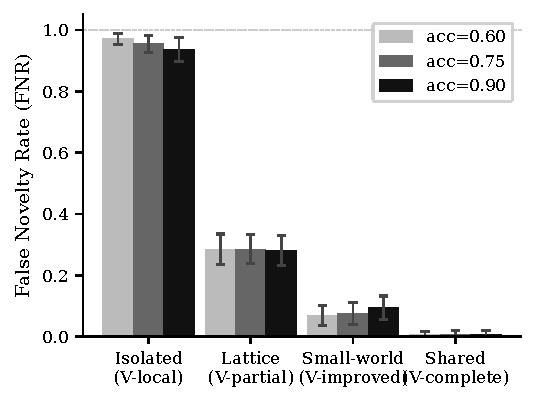
\includegraphics[width=0.72\columnwidth]{fig_fnr_primary_n30.pdf}
\caption{False novelty rate (FNR) by $V$-completeness level (connectivity condition) and classifier accuracy. Error bars show $\pm 1$ std across 30 seeds ($n=200$ hypotheses, 40 latent classes, 20 agents). Across conditions the FNR span is $0.947$; within any condition varying classifier accuracy over 0.60--0.90 moves FNR by $\leq 0.035$. Both ranges are sensitive to their chosen endpoints and are reported descriptively.}
\label{fig:fnr}
\end{figure}

An additional robustness sweep varying the hypothesis space complexity ($n_\text{latent} \in \{20, 40, 80\}$) reveals that the magnitude scales with domain complexity: isolated agents achieve FNR $=0.642$ at 20 latent classes (a simple domain where local memory frequently saturates), but FNR rises to $0.995$ at 80 classes. Medium-connectivity ($k\approx 4$) deteriorates similarly (FNR $0.002 \to 0.292$), while shared topology remains near zero across all complexity levels---consistent with the structural account and not independently informative about emergent dynamics. The failure mode is more severe in complex domains such as biology and mathematics (Table~\ref{tab:domain-comparison}) than in constrained settings such as formal verification.

\textbf{Limitations.} This simulation uses synthetic agents and a ground-truth novelty oracle unavailable in real science; its agents do not generate hypotheses, run experiments, or update beliefs. The connectivity-to-$V$-completeness mapping is an operationalization, not an identity. As noted in the Results, the FNR--recall tradeoff is structurally determined: the mechanism (memory union growth with degree) cannot produce any outcome other than the one reported, and the simulation is therefore an existence illustration rather than an empirical measurement. The effect magnitude further depends on the prior seeding rate: the FNR ordering (more connected $\to$ lower FNR) is robust across 2--20\% seeding rates, but absolute differences collapse above 10\% seeding and balanced accuracy ordering reverses, confirming that no coverage-based topology achieves stable discrimination across prior-knowledge regimes. The simulation is intended to make the structural consequence of $V$ incompleteness legible, not to measure its magnitude in any deployed system.

\section{Open Problems}
\label{sec:openproblems}

Our analysis identifies three open problems that persist across all systems and domains.

\subsection{The Non-Automatability of Novelty}

Every system in our survey encounters the same problem: novelty cannot be reliably evaluated by automated means. The trajectory of systems from Coscientist (no mechanism) to The AI Scientist Nature (three-layer validation including actual peer review) converges on the same conclusion; ARA~\citep{liu2026lasthuman} makes this an explicit design principle, reserving significance, novelty, and taste for human reviewers while automating the mechanical layers of review.

Two specific failure modes are documented: (1) \emph{LLM self-evaluation bias}, manifesting as systematic over-estimation of novelty and quality ($+$2.3 points in Agent Laboratory; hallucinated results in The AI Scientist Sakana; grade inflation observed in 17/23 ARA artifacts despite structural safeguards); and (2) \emph{pretraining contamination}, most acutely in mathematics, where systems may ``discover'' results implicit in their training data (as documented by Aletheia for Erd\H{o}s problems).

The ARA Seal~\citep{liu2026lasthuman} represents the most concrete existing proposal for automating the sub-novelty layers of $V$: its Rigor Auditor detects 82.6\% of seeded structural violations across five injection types, with a documented 22\% blind spot for orphaned experiments. This calibrates how far automated verification can reach before the novelty boundary. Addressing the boundary itself requires either evaluation protocols robust to pretraining contamination, or explicit architectural separation between the generating model and the evaluating model---approaches that remain largely unexplored.

\subsection{The BED--Practice Gap for $\pi$}

Equation~\ref{eq:eid} specifies the theoretically optimal search policy: select the experiment that maximizes EIG. The theoretical infrastructure for approximating this policy exists~\citep{foster2019variational,foster2021dad,blau2022rl}, yet no current AI Scientist system implements it. Instead:

\begin{itemize}
  \item Coscientist: reactive ($\pi$ = next tool selection)
  \item AI Scientist Sakana: greedy ($\pi$ = avoid archive similarity)
  \item AI Scientist Nature: best-first tree search (node scoring by GPT-4o)
  \item Agent Laboratory: sequential (human-guided)
  \item GNoME: uncertainty sampling ($\pi \approx$ EIG proxy over GNN posterior) --- the closest approximation, but restricted to domains with tractable probabilistic models
\end{itemize}

The gap between available theory and deployed practice is striking, though one partial exception exists. GNoME's~\citep{merchant2023gnome} uncertainty-sampling policy---prioritizing crystal structures where the GNN stability prediction has highest entropy---is structurally equivalent to information-gain maximization over a probabilistic model. It approximates EIG without computing it explicitly, by treating GNN uncertainty as a proxy for posterior entropy $H(\theta \mid b)$. This works in materials science because $V_\text{empirical}$ (DFT) is well-calibrated and the GNN posterior is tractable. In LLM-based systems, neither condition holds: the ``posterior'' over hypotheses is implicit in language model weights, and EIG requires integrating over $p(\theta \mid y)$, which is intractable without significant architectural changes. Amortized EIG approximations~\citep{foster2021dad} that use trained neural networks to estimate information gain efficiently may offer a viable path forward for domains where a tractable model of the hypothesis space can be maintained.

\subsection{The Underdevelopment of Semantic Memory $M_s$}

Current systems predominantly implement $M_e$ (episodic memory: storing raw experiment records). $M_s$ (semantic memory: distilled patterns and regularities extracted from experimental history) is largely absent. The consequence is that a system with 1,000 completed experiments does not search more intelligently than one with 10, because accumulated experience is not distilled into improved $G$ or $\pi$.

The cost of this absence is empirically visible in the reproducibility gap. \citet{liu2026lasthuman} report that 90.2\% of the dollar cost of extending a published result is consumed by failed rediscovery---reconstruction of intermediate knowledge the original authors possessed but did not publish. This is precisely the knowledge that $M_s$ should encode but does not: the dead ends, pivots, and hard-won heuristics that distinguish experts from novices.

The ARA \texttt{/trace} layer~\citep{liu2026lasthuman} is the closest existing approximation: it encodes the exploration graph with typed nodes (experiment, dead\_end, pivot) and forensic bindings to evidence. However, this is a representation framework rather than a learning mechanism---$M_s$ is structured but not automatically distilled from experimental outcomes. Empirically, preserved traces accelerated agent performance on extension tasks but also anchored more capable agents to prior solution paths, suggesting that $M_s$ structure must be paired with mechanisms for selectively forgetting or abstracting over low-level history.

Building systems where $G(M_s, S)$ genuinely improves with accumulated experience---not merely by appending to an archive but by distilling transferable knowledge---is an open problem with significant implications for long-horizon scientific discovery.

\section{Discussion}
\label{sec:discussion}

\textbf{Implications for system design.} Our analysis suggests a design hierarchy: the choice of $V$ should precede all other design decisions, as it determines whether closed-loop operation is feasible and what form $\pi$ can take. Domains where $V$ is approximated by noisy surrogates (chemistry, biology) require $\pi$ strategies that are robust to reward noise---a requirement that beam search partially addresses (ChemReasoner) but that has not yet been systematically studied.

\textbf{The role of human oversight ($H$).} Rather than treating $H$ as a limitation to be minimized, our analysis suggests that explicit human integration at the $\pi$ and $V_\text{human}$ level is not only practically necessary but theoretically well-motivated. In the POMDP formulation, human judgment provides access to a richer information source than any automated proxy, particularly for the non-automatizable components of $V$ (novelty, significance). Systems that design $H$ explicitly, as in The Last Human-Written Paper, may achieve better outcomes than those that attempt to minimize it.

\textbf{Towards collective AI co-scientists.} All systems analyzed in this survey operate as single-agent loops. A natural extension is a \emph{collective} AI scientist: a multi-agent system $\{$\framework$_k\}_{k=1}^K$ sharing an external semantic memory $w$ and coordinating through a collective validator $V_\text{collective}$. \citet{taniguchi2024cpc} formalize this vision via Collective Predictive Coding, recasting science as decentralized Bayesian inference in which a community of agents with diverse priors $\theta_k$ jointly updates a shared representation $w$ through experimentation and peer review modeled as a Metropolis-Hastings consensus process. In their framework, social objectivity emerges from prior diversity---a requirement that LLM-based systems currently fail, since all instances share the same pretraining distribution. This is the ``communication barrier'' that \citet{taniguchi2024cpc} identify as the central obstacle to AI participation in collective science, and it constitutes a fourth open problem beyond the three we identify.

Notably, the three open problems in our analysis are precisely the necessary conditions for a collective AI co-scientist to be realizable: $V_\text{collective}$ requires solving novelty automatability; a principled collective $\pi$ requires closing the BED--practice gap; and the shared $w$ requires a developed $M_s$. Their convergence suggests that progress on any one of the three would unlock disproportionate gains toward the collective system---and that ARA~\citep{liu2026lasthuman}, as a structured artifact protocol for $w$, may be the most tractable entry point.

\textbf{Limitations.} Our framework \sgmvpi{} abstracts away important domain-specific nuances, including the cost structure of $E$ (which varies by orders of magnitude across domains), the non-stationarity of $S$ (open-ended problems), and the distinction between single-task and multi-task discovery. The single-agent framing also abstracts away the social layer that \citet{taniguchi2024cpc} formalize; extending \framework{} to multi-agent settings is a natural direction for future work.

\section{Conclusion}
\label{sec:conclusion}

We introduced \framework{}, a formal framework \sgmvpi{} for characterizing AI Scientist systems, and applied it to four core end-to-end systems, one artifact infrastructure proposal, and domain-specific instantiations across seven scientific fields. The framework connects the AI Scientist literature to the established theories of POMDPs and Bayesian Experimental Design, providing a principled basis for evaluating and improving search policies.

Three findings stand out from the cross-system, cross-domain analysis. First, current AI Scientist systems are best understood as a progression toward more complete validators: every architectural advance---from Coscientist's single-measurement $V_\text{human}$ to The AI Scientist's automated reviewer to GNoME's DFT oracle---is ultimately a gain in $V$ completeness, and $V$ completeness is what unlocks closed-loop operation. Second, the BED--practice gap for $\pi$ is real but not absolute: GNoME's uncertainty-sampling policy approximates EIG in a tractable probabilistic setting, showing that the gap is a solvable engineering problem in domains where a learnable model of the hypothesis space exists. Third, the underdevelopment of $M_s$ is the least-addressed bottleneck: systems can close their loops with $M_e$ alone, but they cannot compound accumulated knowledge without distillation---a capability that determines whether AI Scientist systems remain expensive one-shot tools or become genuinely cumulative research partners.

The three open problems we identify---novelty non-automatability, the BED--practice gap, and $M_s$ underdevelopment---are not independent. A system with complete $V$ and tractable $M_s$ would, by construction, be able to implement an EIG-optimal $\pi$. The convergence of all three problems on the same structural gap suggests a single organizing question for the field: \textit{how do we build validators and memory structures that are simultaneously complete enough to support closed-loop operation and structured enough to support principled search?}

\bibliographystyle{abbrvnat}
\bibliography{references}

% ---------------------------------------------------------------
\newpage
\section*{AI Involvement Checklist}
\label{sec:ai-checklist}

This checklist documents the role of AI systems at each stage of this research, as required by CAISc 2026.

\begin{itemize}
  \item \textbf{Hypothesis development.} The core \framework{} framework \sgmvpi{}, the $H$ parameter, the $G$ output spectrum (propositional hypothesis $\to$ falsifiable construction), and the three open problems were conceived by the human author. Claude Code (Anthropic) elaborated framework components, identified paper-level instantiations of each component, and proposed connections between concepts.

  \item \textbf{Literature search and selection.} The human author determined inclusion criteria and target systems. Claude Code autonomously retrieved and read over 40 full-text PDFs, categorized papers into the taxonomy, and performed claim-level verification against source text.

  \item \textbf{Analysis.} Claude Code extracted S, G, E, V, M, $\pi$ components for each of the 13 analyzed systems by reading primary sources. The human author reviewed all extractions, corrected mischaracterizations (several substantive corrections were required), and synthesized cross-system patterns.

  \item \textbf{Writing.} Claude Code drafted the majority of this manuscript. The human author provided key conceptual passages (notably \S\ref{sec:open-problems} and the core definitions in \S\ref{sec:framework}), directed structural decisions, and reviewed all drafts.
\end{itemize}

\noindent Overall, the division of labor is best characterized as: the human author provided intellectual direction, framework design, and final judgment; Claude Code provided literature retrieval, analysis execution, and text generation.

% ---------------------------------------------------------------
\newpage
\section*{Responsibility \& Reproducibility Checklist}
\label{sec:repro-checklist}

\begin{itemize}
  \item \textbf{Claims and evidence.} All empirical claims are grounded in cited primary sources. Major claims were verified by direct full-text reading of source PDFs; specific figures (e.g., Science of Science statistics) were cross-checked against institutional press releases where journal access was unavailable.

  \item \textbf{Limitations.} This paper is a conceptual meta-analysis of existing published systems. It contains no original experiments. The \framework{} framework is not empirically validated against held-out systems in this submission; its descriptive adequacy rests on consistency across the 13 analyzed systems. Domain-specific cost structures, multi-agent dynamics, and temporal evolution of systems are not modeled.

  \item \textbf{Reproducibility.} The analytical framework can be applied to any AI Scientist system following the component definitions in \S\ref{sec:framework}. All analyzed papers are publicly accessible. No proprietary data or closed models were used.

  \item \textbf{Experimental details.} Literature review methodology follows Muka et al.\ (2020) 24-step systematic review guide. System selection criterion: end-to-end automation of at least one component of the hypothesis--experiment--validation loop.

  \item \textbf{Data and code availability.} Analysis notes will be made available upon acceptance. No datasets were produced.

  \item \textbf{Ethical and societal impact.} The $H$ parameter analysis explicitly addresses the necessity of human oversight in current systems. The Science of Science discussion (\S\ref{sec:open-problems}) flags risks of research homogenization under widespread AI Scientist deployment, citing empirical evidence from Park et al.\ (2023) and Wu et al.\ (2019).
\end{itemize}

\end{document}
